\section{Implementacion}\label{sec:implementacion}

\subsection{Simulacion}\label{subsec:simulacion}

    En lo que refiere a la simulacion del modelo, esta diseñado para trabajar con automatas de tres dimensiones, ya que
    toda posicion (Ver clase Position en el UML~\ref{fig:UML-Simulacion}) comprende las componentes x, y, z. En caso de ser
    bidimensional, toda posicion tendra $z = 0$.


%\begin{wrapfigure}{r}{0.6\textwidth}
%    \centering
%    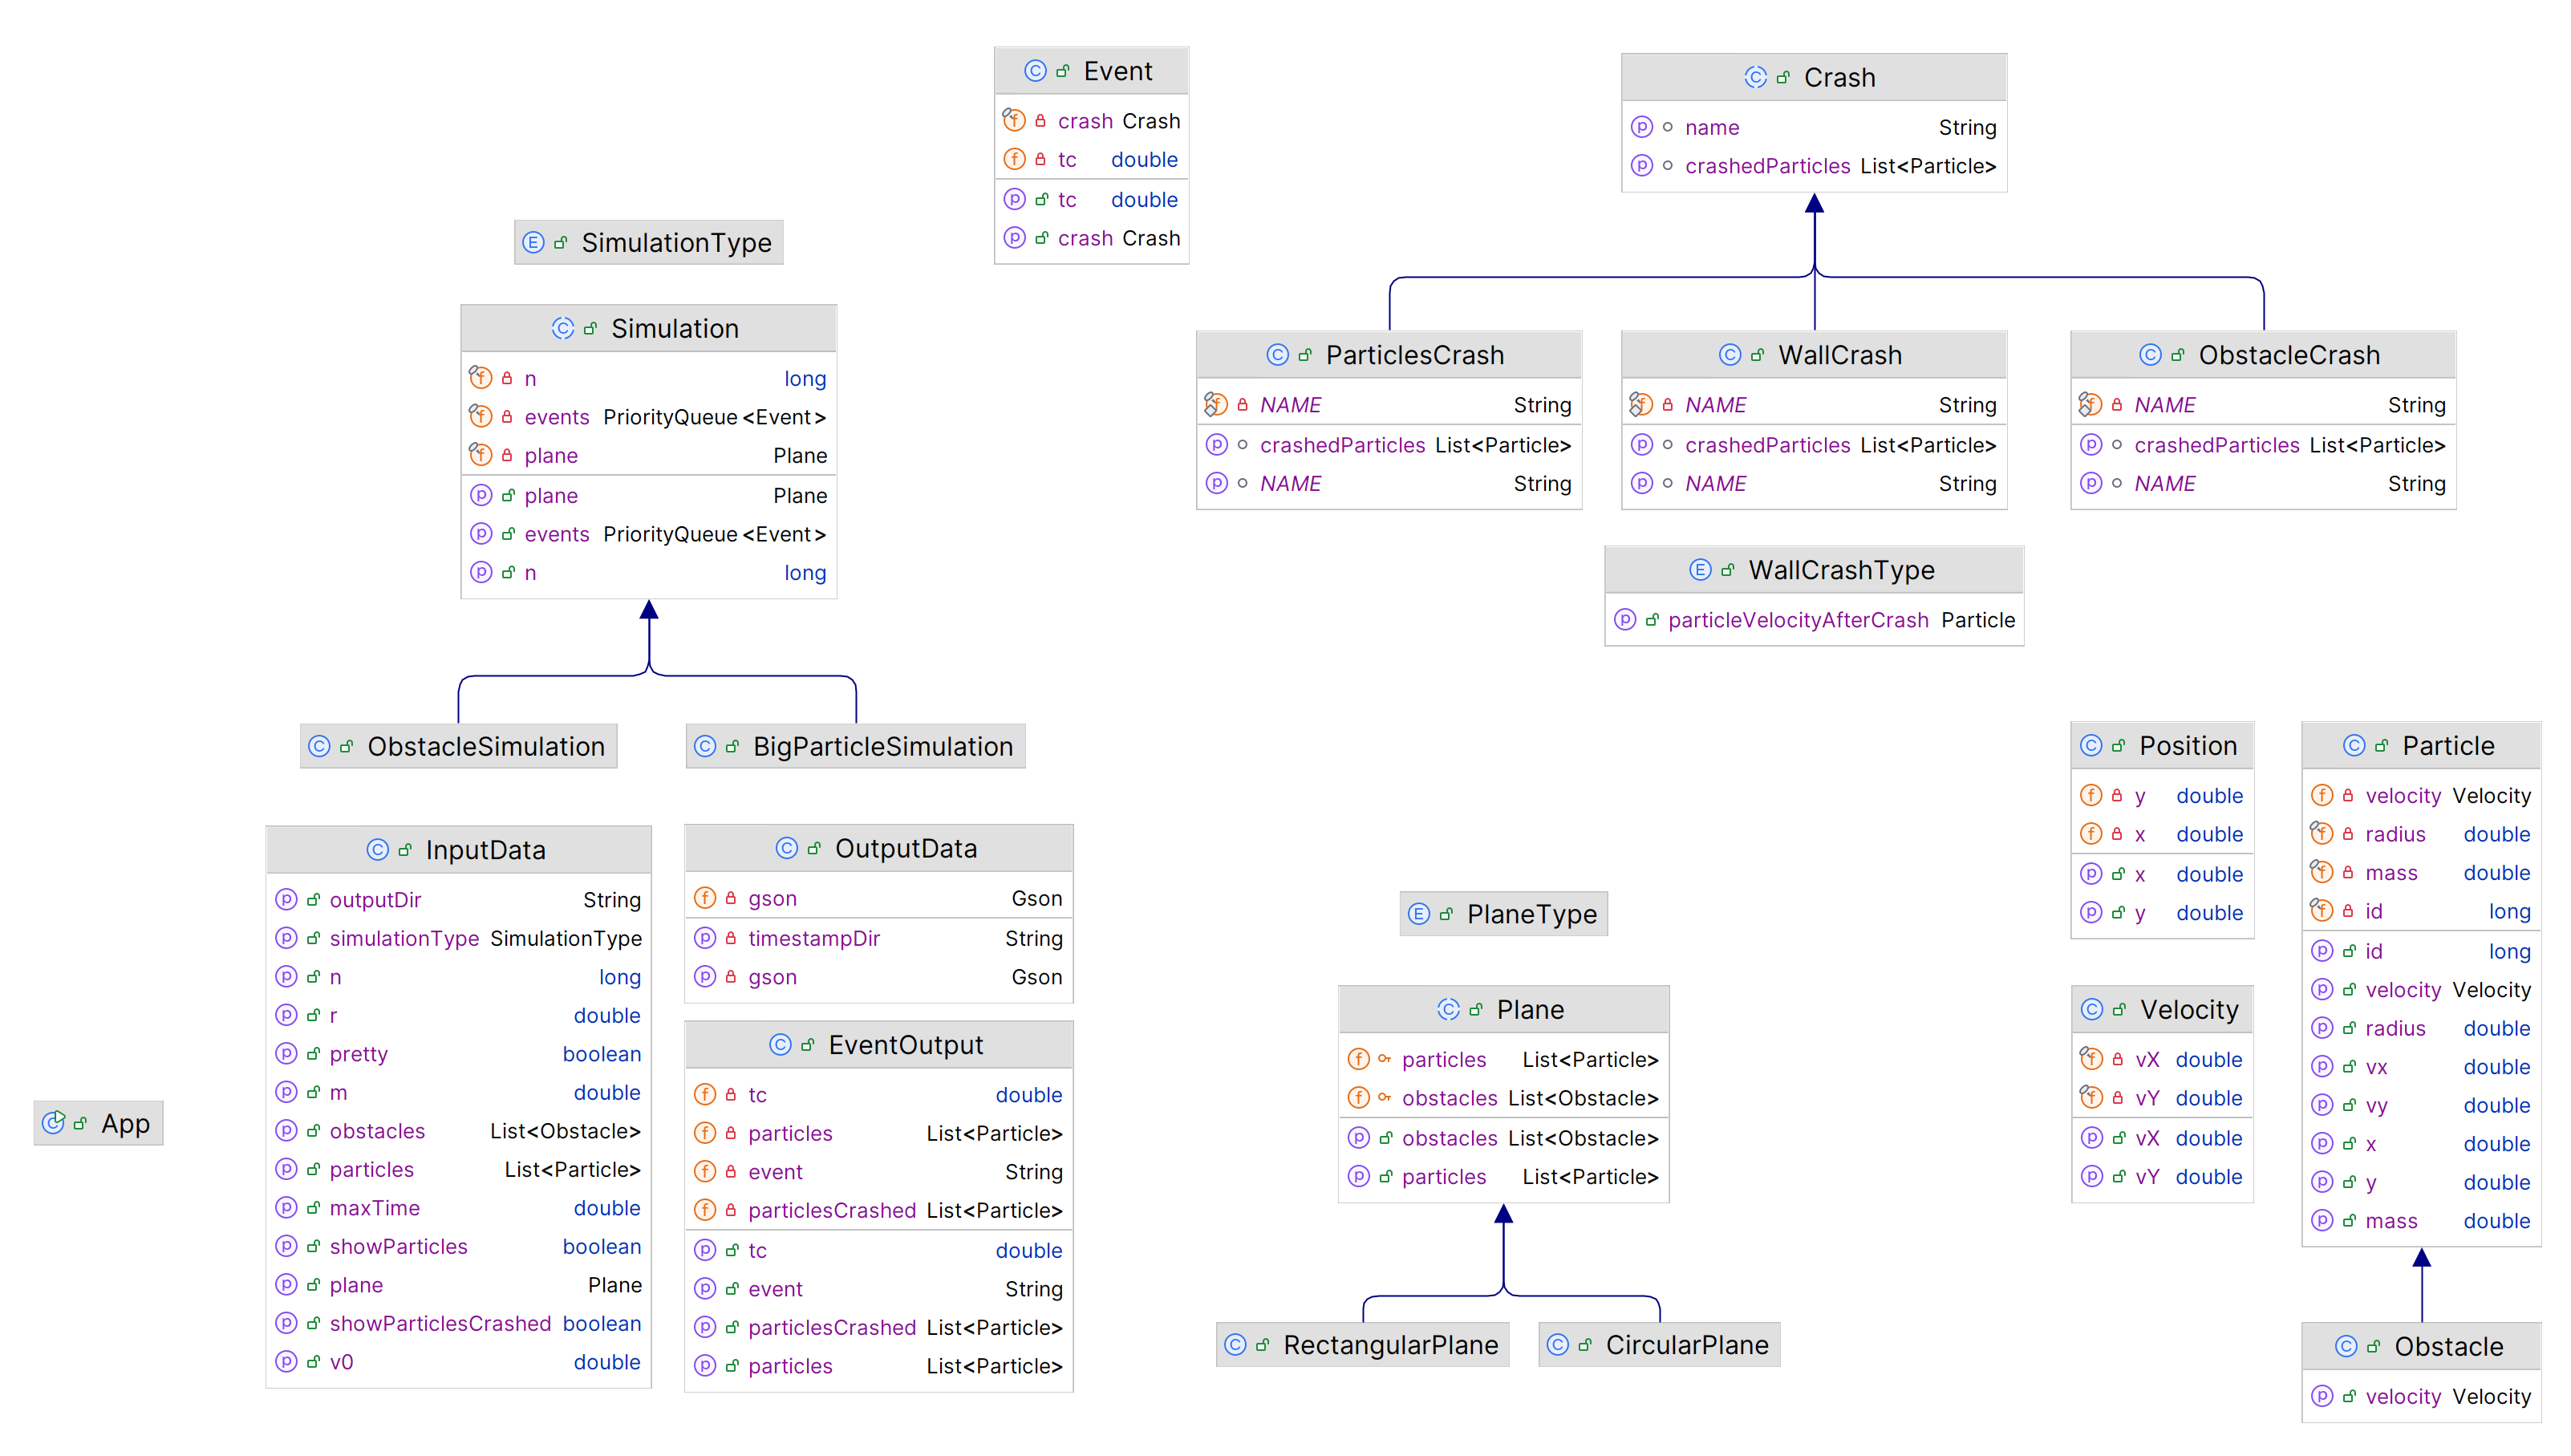
\includegraphics[width=1\linewidth]{UML}
%    \caption{Diagrama UML}
%    \label{fig:UML-Simulacion}
%\end{wrapfigure}

\begin{figure}[H]
    \centering
    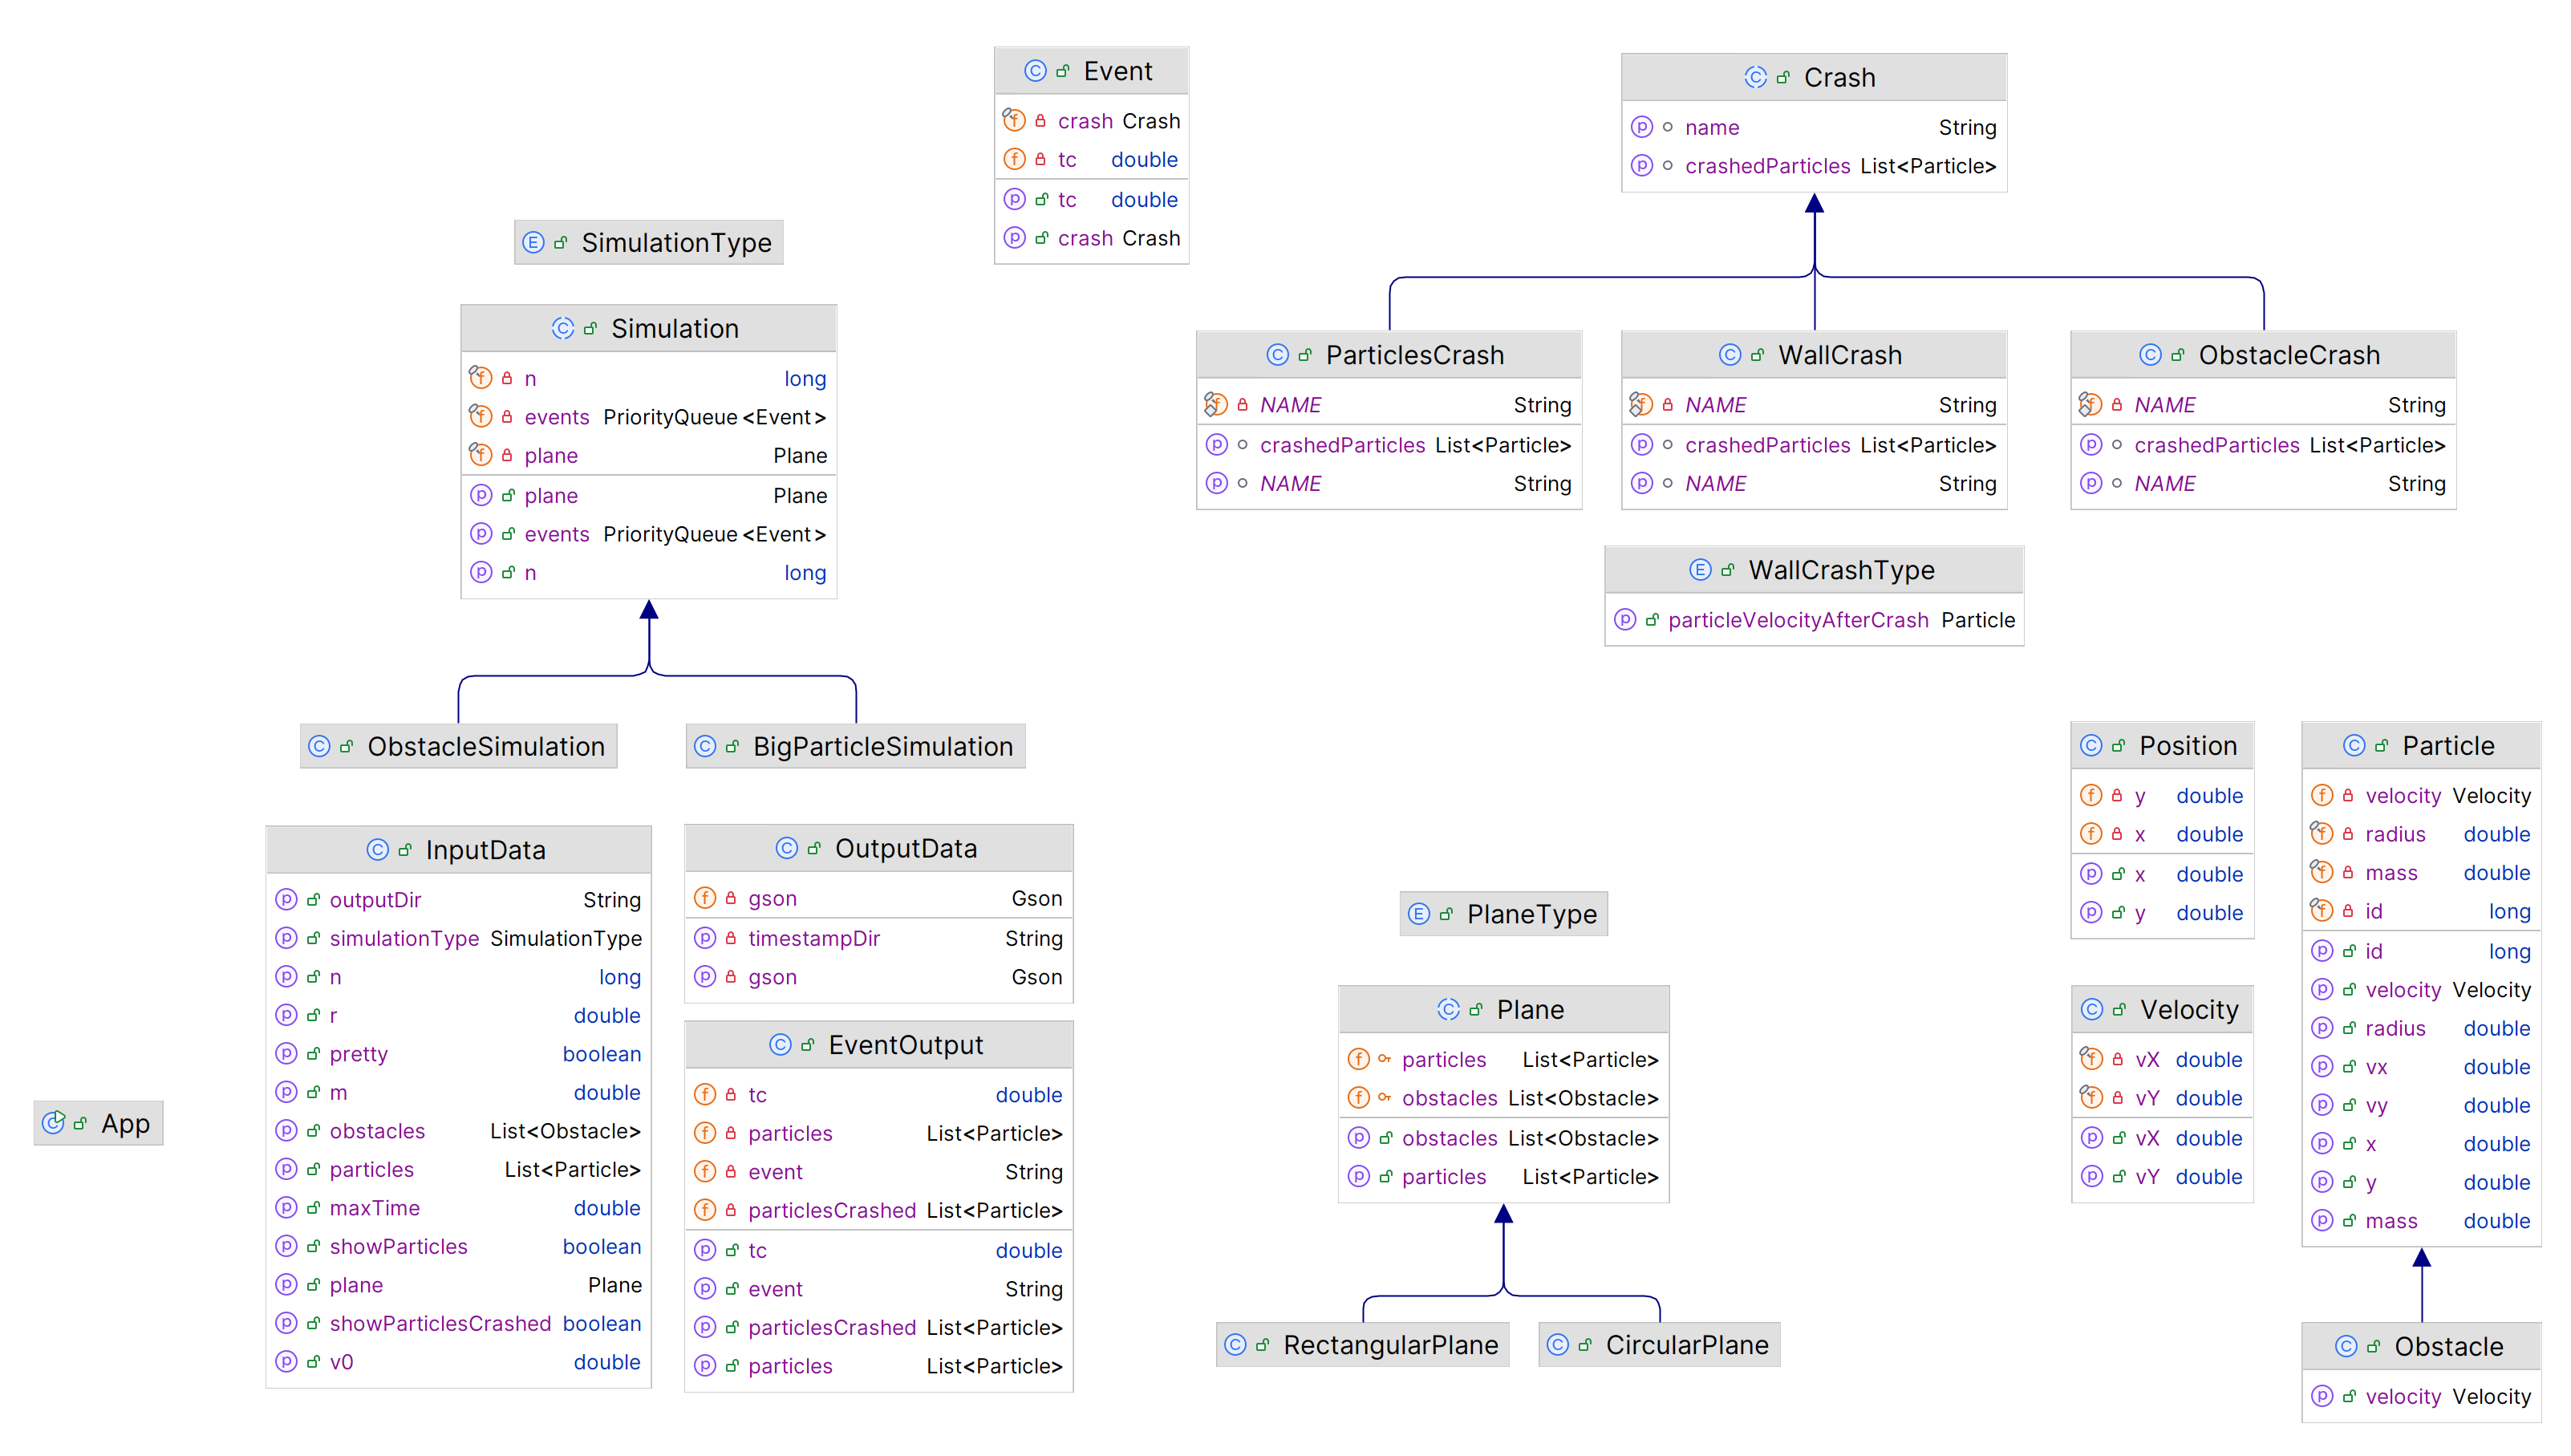
\includegraphics[width=1\linewidth]{UML}
    \caption{Diagrama UML de codigo Java de simulacion}
    \label{fig:UML-Simulacion}
\end{figure}
